\chapter{Umsetzung des Projektes}
\section{Komponenten und Aufbau}
\label{sec:Peri}
Das Projekt wird auf einem Arduino Micro umgesetzt. Dieser ist ein Entwicklerboard, basierend auf dem Mikrocontroller ATmega32U4. Er wird mit 16MHz getaktet und 5V betrieben. Der Programmspeicher umfasst 32KB. Weiterhin besitzt der Controller 2.5KB SRAM als Arbeitsspeicher sowie 1KB EEPROM für dauerhaftes Speichern von Werten.
Die Steuerung des Spiels erfolgt über Joysticks, dessen Position über Potentiometer in eine Spannung abgebildet wird. 
Die Anzeige erfolgt über ein 4-Zeilen Display (Modell 2004) mit parallelem Interface. Ein FC-113 I2C-Brückenchip wandelt die seriell über I2C gesendeten Displaykommandos in das parallel Interface um. Das Programm wird mittels Programmer EvUSBasp auf den Controller geladen. Im Folgenden sind die verwendeten Komponenten aufgezählt:
\begin{itemize}
\setlength\itemsep{-0.5em}
\item Arduino Micro
\item I2C Displayinterface FC-113 
\item 4-Zeilen LC-Display Modell 2004
\item 2 $\times$ Potentiometer-Joystick
\item EvUSBasp USB-Programmer
\end{itemize}

Abbildung \ref{fig:Aufbau} zeigt den Aufbau des Projektes.
\begin{figure}[H]
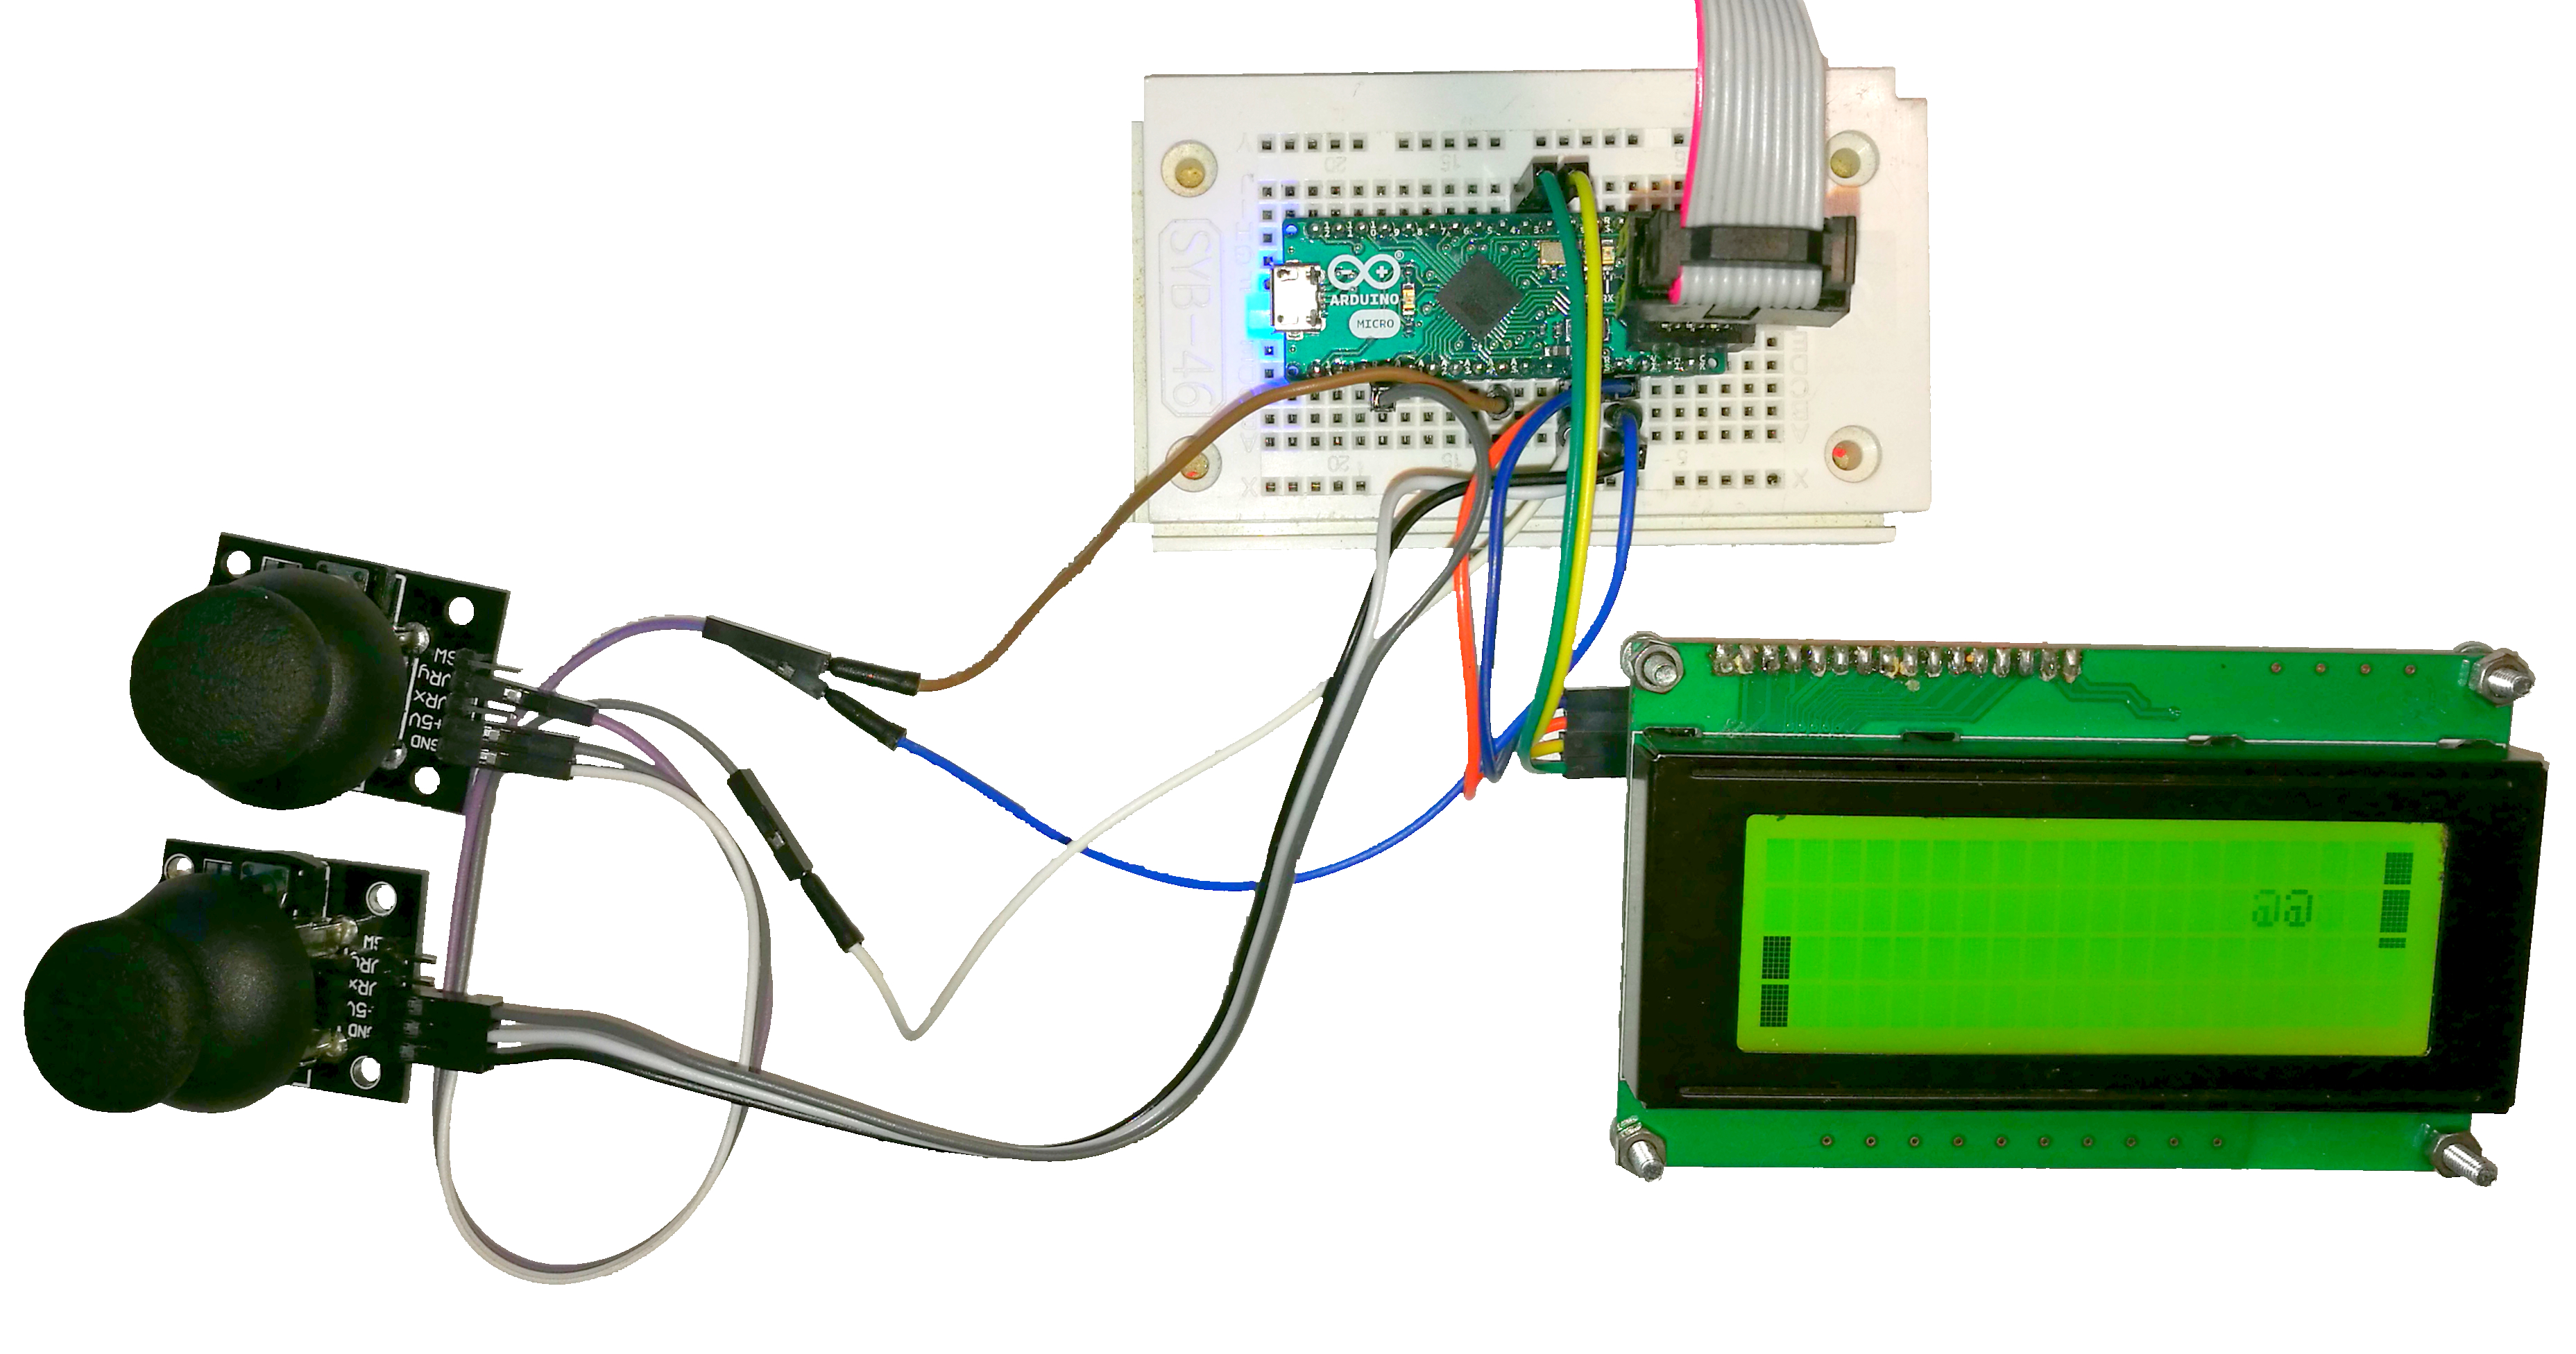
\includegraphics[width=\textwidth]{./Bilder/Aufbau.jpg}
\caption{Aufbau des Projektes}
\label{fig:Aufbau}
\end{figure}

Die nachfolgende Tabelle listet die Pinbelegung des Arduino Micro in diesem Projekt. Die Massepins und Versorgungsspannungen wurde für bessere Übersichtlichkeit ausgelassen.

\begin{table}[H]
\begin{center}
\caption{Pinbelegung}
\begin{tabular}{|c|c|}
\hline 
Komponente & Pin am Arduino \\ 
\hline
\hline 
Joystick 1 - Teilerspannung & A5 \\ 
\hline 
Joystick 2 - Teilerspannung & A0 \\ 
\hline 
Display - I2C SDA & D2 \\ 
\hline 
Display - I2C SCL & D3 \\ 
\hline 
\end{tabular}
\end{center}
\end{table}
%Pinout nennen

\section{Entwicklungsumgebung}
\label{sec:IDE}
Die zur Programmierung des ATmega32U4 unter Linux Ubuntu notwendigen Programme werden mittels Paketverwaltung \glqq apt\grqq\ installiert:
\begin{itemize}
\setlength\itemsep{-0.5em}
\item Es wird der ATmega-kompatible C-Compiler \glqq avr-gcc\grqq\ genutzt.
\item Für den Flash-Vorgang ist die Programmiersoftware \glqq avrdude\grqq\ notwendig.
\item Die automatische Kompilation und das Linken wird durch die Software \glqq Make\grqq\ verwaltet. Dazu wird ein sog. \glqq Makefile\grqq\ erstellt (siehe Abschnitt \ref{sec:Make}).
\item Zur Erstellung des Quelltextes wird der Editor \glqq Visual Studio Code\grqq\ eingesetzt.
\item Der Programmer USBasp konnte ohne Installation von zusätzlichen Treibern eingesetzt werden.
\end{itemize}
\noindent Die Wahl des Editors fiel auf Visual Studio Code, da dieser Abhängigkeiten, sowie C-Syntax überprüfen kann. Die Integration von Intellisense als Algorithmus hinter der Autovervollständigung ermöglicht effizientes Verfassen von Quelltexten. Die nachfolgende Abbildung zeigt die Oberfläche von Visual Studio Code.

\begin{figure}[H]
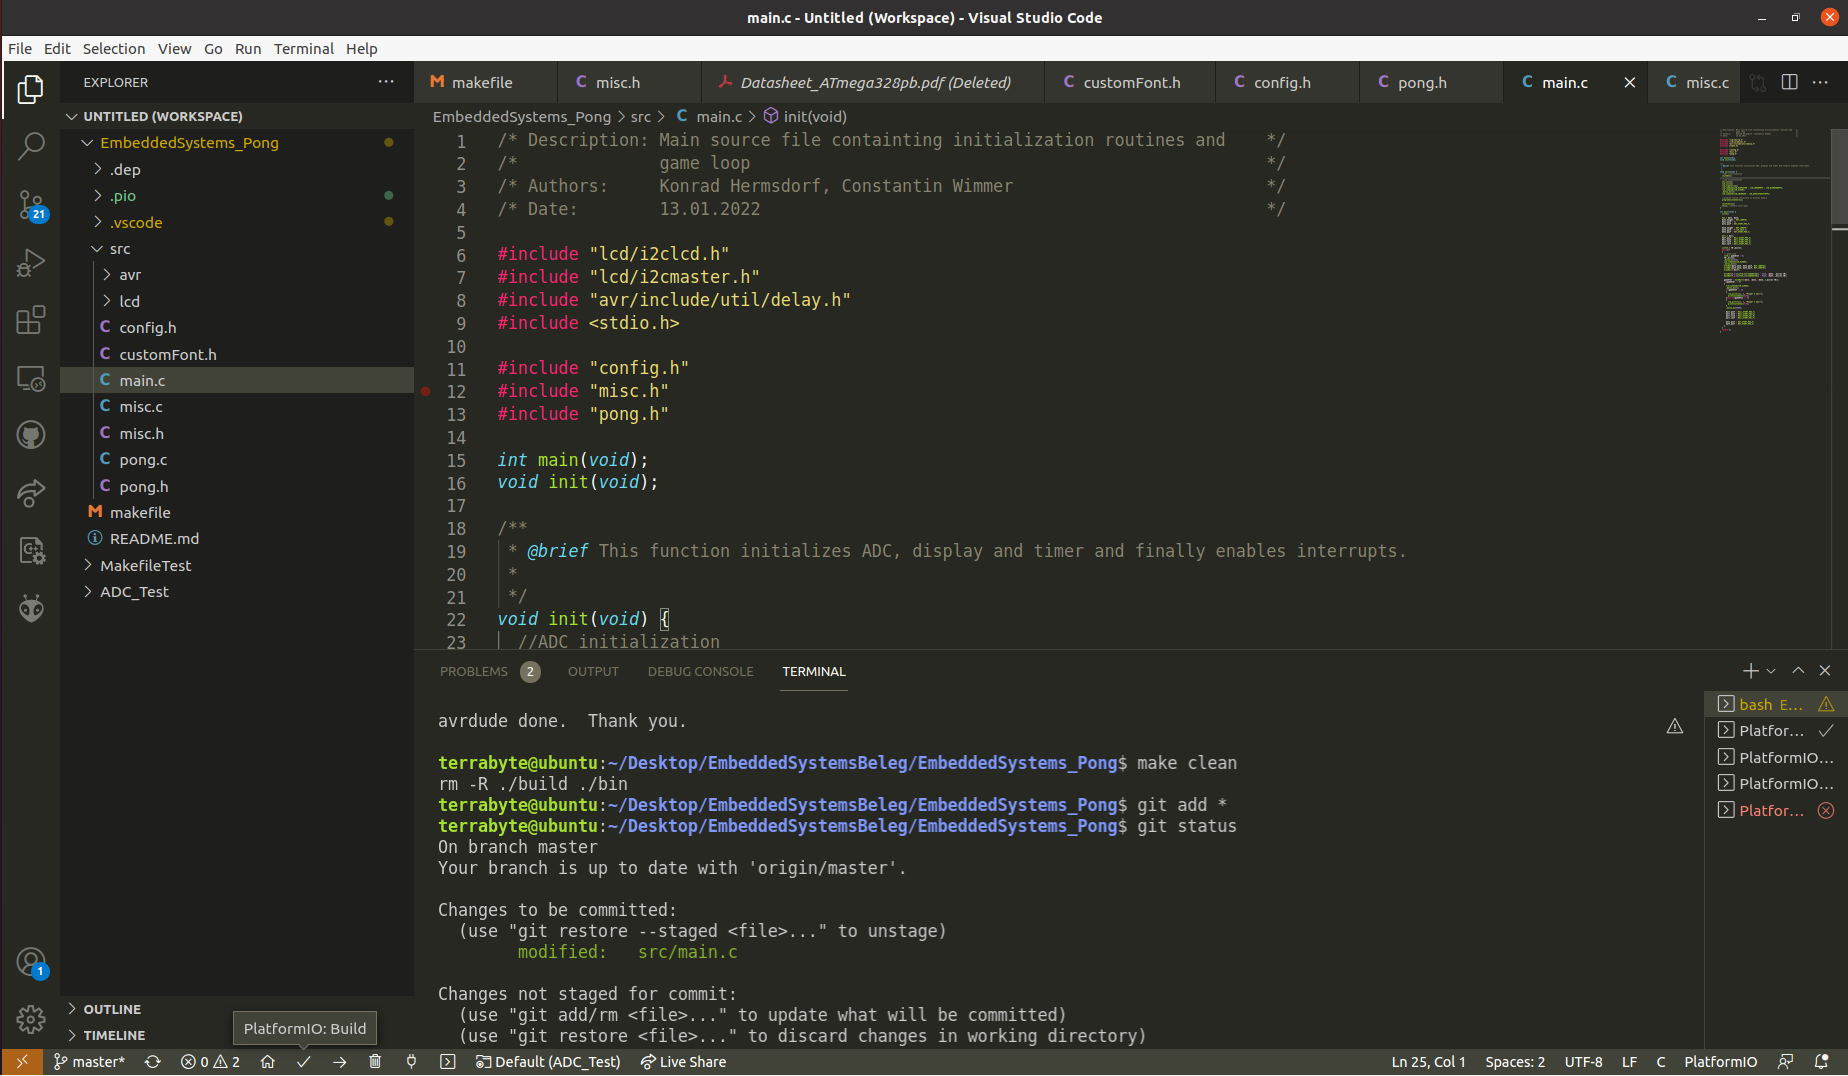
\includegraphics[width=\textwidth]{./Bilder/Code.png}
\caption{Oberfläche von Visual Studio Code}
\end{figure}


\section{Programmstruktur}
\label{sec:Prog}
Das Programm lässt sich grob in die Aufgabenbereiche Spielschleife, Zeichenroutinen und Verwaltung der Peripherie einteilen. Nach einer anfänglichen Initialisierungsphase, wird in der Spielschleife zyklisch die Position der Joysticks über den ADC-Wert abgefragt. Dieser Wert wird genutzt, um die Position der Ankerpunkte der Schläger im nächsten Bild zu berechnen. Bei Berechnung der Ballposition wird beachtet, ob der Ball hinter einem Schläger gelandet ist oder eine Wand berührt hat in erstem Fall wird eine Siegesnachricht angezeigt, in letzterem Fall die y-Richtung des Balls umgekehrt. Bei Berührung eines Schlägers wird die x-Richtung umgekehrt.\\
Die Größe der Bewegung je Bild für Ball und Schläger wird außerdem proportional zur verstrichenen Zeit zwischen zwei Bildern festgelegt. Dazu wird Timer 1 des ARmega32U4 zur Auslösung einer Interrupt-Service-Routine eingesetzt, welche eine Variable inkrementiert, die die Verstrichenen Mikrosekunden seit Timer-Start speichert.\\
Die Ansteuerung des Displays erfolgt über den Laborunterlagen entnommenen Programmcode. Dieser erlaubt die Programmierung eigener Schriftzeichen im Display. Das wurde genutzt um je Displayzeile 4 verschiedene Schlägerpositionen darstellen zu können.
Eine ausführliche Dokumentation aller Funktionen findet sich im Anhang \ref{cha:Doxy} in Form einer Doxygen-generierten Quelltextbeschreibung.

\section{Automatische Maschinencodeerstellung mittels Makefile}
\label{sec:Make}


 

